\chapter{Interactive tools}

\section{Generalities}

%Generate with make input.

%=======================================
\section{Entering mask with {\tt SaisieMasq} or {\tt SaisieMasqQT} }

\subsection{SaisieMasq}

{\tt SaisieMasq} is a very simple tool to edit mask images.
It creates a binary mask image from a polygonal selection in the displayed image.\\*

Typing {\tt SaisieMasq -help}, one gets:

\begin{verbatim}
*****************************
*  Help for Elise Arg main  *
*****************************
Unamed args :
  * string :: {Name of input image}
Named args :
  * [Name=SzW] Pt2di
  * [Name=Post] string
  * [Name=Name] string :: {Name of result, default toto->toto_Masq.tif}
  * [Name=Gama] REAL
  * [Name=Attr] string
\end{verbatim}

Meaning of args is:

\begin{itemize}
   \item First arg: pattern specifying the images to load (can be 1 or more images) - regular expression are supported;
   \item optional {\tt SzW}, def = [$900,700$], size of display window;
   \item optional {\tt Post}, def = "Masq" , postfix to add to output filename;
   \item optional {\tt Name}, name of result;
   \item optional {\tt Gama}, def = $1.0$ , gama applied to images, it can help with dark images, or wide dynamics;
   \item optional {\tt Attr}, text to add to postfix;\\*
\end{itemize}


Processing is as follow:
\begin{itemize}
\item Click: add a point to polygon
\item Shift click: close polygon and apply selection
\item Ctrl + right click: delete last point
\item Shift + right click + Coul : switch between add mode and remove mode
\item Shift + right click + Exit : save mask image and {\tt Xml} file and quit
\end{itemize}

\subsection{SaisieMasqQT}

\label{Doc:SaisieMasqQT}
{\tt SaisieMasqQT} is the same tool as {\tt SaisieMasq}, available on all platforms (Linux, Windows, MacOS).
{\tt SaisieMasqQT} can be run several ways. You can run command {\tt mm3d SaisieMasqQT} and drag-and-drop files in the application window, or open files from File menu, or you can run command {\tt mm3d SaisieMasqQT + arguments}\\*

Example: {\tt mm3d SaisieMasqQT IMG.tif SzW=[1200,800] Name=PLAN Gama=1.5}\\*

You can also run command {\\ mm3d SaisieMasqQT -l} to load last edited file.
A visual interface for argument edition is also available with command: {\tt mm3d vSaisieMasqQT}
As usual, type {\tt mm3d SaisieMasqQT -help}, to get help message.\\*

{\tt SaisieMasqQT} has the same arguments as SaisieMasq. Some light differences with {\tt SaisieMasq} processing workflow should be noticed:
you need to draw a polygon first, and then apply an action (add to mask, remove from mask, etc.).
You can get a complete list of possibles actions typing F1.\\*

Main actions are:
\begin{itemize}
\item F2: display image in full screen
\item Wheel roll: zoom
\item Wheel click: move image
\item Shift+wheel click: zoom fast
\item Left click: add a point to polygon
\item Right click: close polygon
\item Space: Add to mask
\item Suppr: Remove from mask
\item Right click (close to a point): delete point
\item Echap: delete polygon
\item Shift + click \& drag: insert point
\item Ctrl+S: save mask image and {\tt Xml} file
\item Ctrl+Q: quit\\*
\end{itemize}

Some parameters can be edited in the {\tt Settings} menu: image gamma, application language, display settings, etc. These parameters are stored, and are used at next application launch, so set them once to fit your own purpose. As SaisieMasqQT can edit both images and 3d point clouds, application has different behavior, depending on which data you deal with. As a result, {\tt Settings} menu, and help window dialog (F1), will change depending on the loaded data. Be careful about this!\\*

Some special features have been added to {\tt SaisieMasqQT}, which may differ from original {\tt SaisieMasq}: 
\begin{itemize}
\item modify current selection, with Shift+Click to insert a point, or Click+drag to move a point
\item modify previous actions, with menu Windows/Show polygons list 
\item measure image distances, with Rule tool\\*
\end{itemize}

To modify previous actions, you can undo/redo last actions with Ctrl+Z/Shift+Ctrl+Z, and you can edit list of previous actions, with menu {\tt Windows/Show polygons list}: click on the actions in the list in the right window, then edit polygon (by adding or moving points), or double-click on the action name (column {\tt Mode}) to change action. Apply changes clicking {\tt Return}, or go in the Menu {\tt Mask edition} and select {\tt Confirm changes}.\\*

Note: if you want to change application language, go in the {\tt Settings} menu, apply changes and restart application.

\section{Entering 3D mask with {\tt SaisieMasqQT} }

{\tt SaisieMasqQT} can also be used to measure 3D mask from a point cloud. This 3D mask is useful to restrict computation to the main object.
{\tt SaisieMasqQT} allows to open ply files in a 3D view and to do a manual segmentation with a polygonal selection tool.
{\tt SaisieMasqQT} can open one or several ply files (provided that ply files have been computed in the same reference frame).
The 3D mask selection with {\tt SaisieMasqQT} is designed to work with some specific functions, such as C3DC: the idea is to do a manual segmentation,
by rotating around the objet, and by drawing a polygon.
Each rotation (or translation) and polygonal selection is stored into a {\tt Xml} file which can be used with other MicMac commands.\\*

Calling SaisieMasqQT can be performed in a command shell with: {\tt mm3d SaisieMasqQT}\\*

To open a ply file, there are 4 possibilities:
\begin{itemize}
\item run command with filename or pattern: {\tt mm3d SaisieMasqQT filename.ply}
\item run command {\tt mm3d SaisieMasqQT} and drag-and-drop ply file(s) in interface
\item run command {\tt mm3d SaisieMasqQT} and use standard open file menu
\item run command {\tt mm3d SaisieMasqQT -l} will open last edited file\\*
\end{itemize}

If input ply filename is {\tt cloud.ply}, resulting {\tt Xml} files are named {\tt cloud\_selectionInfo.xml} and {\tt cloud\_polyg3d.xml}, and are saved in the ply file directory.
The file to be used for parameter {\tt Masq3D} of {\tt C3DC} command is {\tt cloud\_polyg3d.xml}.\\*

User can mainly perform 2 actions:
\begin{itemize}
\item move camera around point cloud (rotate and/or translate and/or zoom)
\item draw a polygon and select/deselect points inside polygon\\*
\end{itemize}

To switch between move mode and selection mode, use F9 key.\\*

To select a part of the point cloud, you have to draw a polygon by clicking in the 3D view. To add a point to the polygon, use left-click, to close the polygon, use righ-click. To select points inside polygon, use space bar.
To change point size, use +/- keys. You can hide or show axis, ball, point cloud bounding box, display point cloud in full screen (F2).
Center point cloud on a vertex by double click on it: next move actions will be done around this point.
Undo/redo last actions with Ctrl+Z/Shift+Ctrl+Z.
You can also modify a selection, with various actions (see help: F1 or previous paragraph: 2D and 3D selection edition work the same way).\\*

For advanced users, {\tt Xml} file format is detailed in \ref{Conv:selection}.

%========================================

\section{Entering points}

 %  -  -  -  -  -  -  -  -  -  -  -  -  -
\subsection{Generalities}


To move into an image, various solutions are proposed in the interface:
\begin{itemize}
\item Click on wheel + move = drag
\item Shift + wheel + vertical move = quick zoom
\item Shift + wheel + horizontal move = slow zoom
\item Wheel roll = zoom
\end{itemize}

\vspace{\baselineskip}
To input points, some menus can be displayed with these shortcuts:
\begin{itemize}
\item Right-click: geometry menu
\item Shift + left-click: info menu
\item Shift + right-click: undo menu
\item Ctrl + right-click: zoom menu
\end{itemize}

\subsubsection{Geometry menu}

This menu can be shown with a right-click:

\begin{figure}[H]
\begin{center}
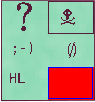
\includegraphics[width=95pt]{FIGS/Saisie/geometry.png}
\end{center}
\label{FIG:button1}
\end{figure}

The corresponding actions are:
\begin{itemize}
\item ;-) validate closest point;
\item (/) invalidate closest point;
\item ? : set point status to dubious
\item skull: don't use closest point
\item HL: highlight point
\item empty box: escape menu (do nothing)
\end{itemize}


\subsubsection{Info menu}

This menu can be shown with Shift + left-click:
\begin{figure}[H]
\begin{center}
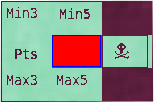
\includegraphics[width=154pt]{FIGS/Saisie/info.png}
\end{center}
\label{FIG:info}
\end{figure}

The corresponding actions are:
\begin{itemize}
\item Pts: select or add a name for this point
\item Min3:
\item Min5:
\item Max3:
\item Max5:
\item skull: delete the point in all images (needs a confirmation)
\item empty box: escape menu (do nothing)
\end{itemize}

\subsubsection{Undo menu}

This menu can be shown with Shift + right-clic:

\begin{figure}[H]
\begin{center}
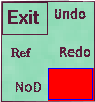
\includegraphics[width=95pt]{FIGS/Saisie/contextual.png}
\end{center}
\label{FIG:contextual}
\end{figure}

The corresponding actions are:

\begin{itemize}
\item Exit: quit the interface, saving {\tt Xml} files
\item Undo: undo last action
\item Redo: redo last action in history
\item Ref: display or not refuted points
\item NoD/Ret: display or not the points names
\item empty box: escape menu (do nothing)
\end{itemize}

\subsubsection{Zoom menu}

This menu can be shown with Ctrl + right-click:

\begin{figure}[H]
\begin{center}
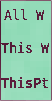
\includegraphics[width=52pt]{FIGS/Saisie/zoom.png}
\end{center}
\label{FIG:zoom}
\end{figure}

The three corresponding actions are:

\begin{itemize}
\item {\tt All W}: full zoom in all windows, and show images where points have not been measured yet;
\item {\tt This W}: zoom only in the window where the menu has been displayed;
\item {\tt This Point}: zoom on the nearest point in all windows where the point is visible
\end{itemize}


 %  -  -  -  -  -  -  -  -  -  -  -  -  -
\subsection{For initial GCP  with {\tt SaisieAppuisInit}}
\label{SaisieAppuisInit}
 %  -  -  -  -  -  -  -  -  -  -  -  -  -

This section describes {\tt SaisieAppuisInit} the graphic interface to input 2D and 3D coordinates of ground control points.

For example with the Saint-Michel de Cuxa data set \ref{Cuxa:DataSet}:

\begin{verbatim}
SaisieAppuisInit  "Abbey-IMG_(021[12]|023[3456]).jpg"  All-Rel  NamePointInit.txt  MesureInit.xml
\end{verbatim}

When running this command, the interface shows data set's first images, where one can point GCPs:

\begin{figure}[H]
\begin{center}
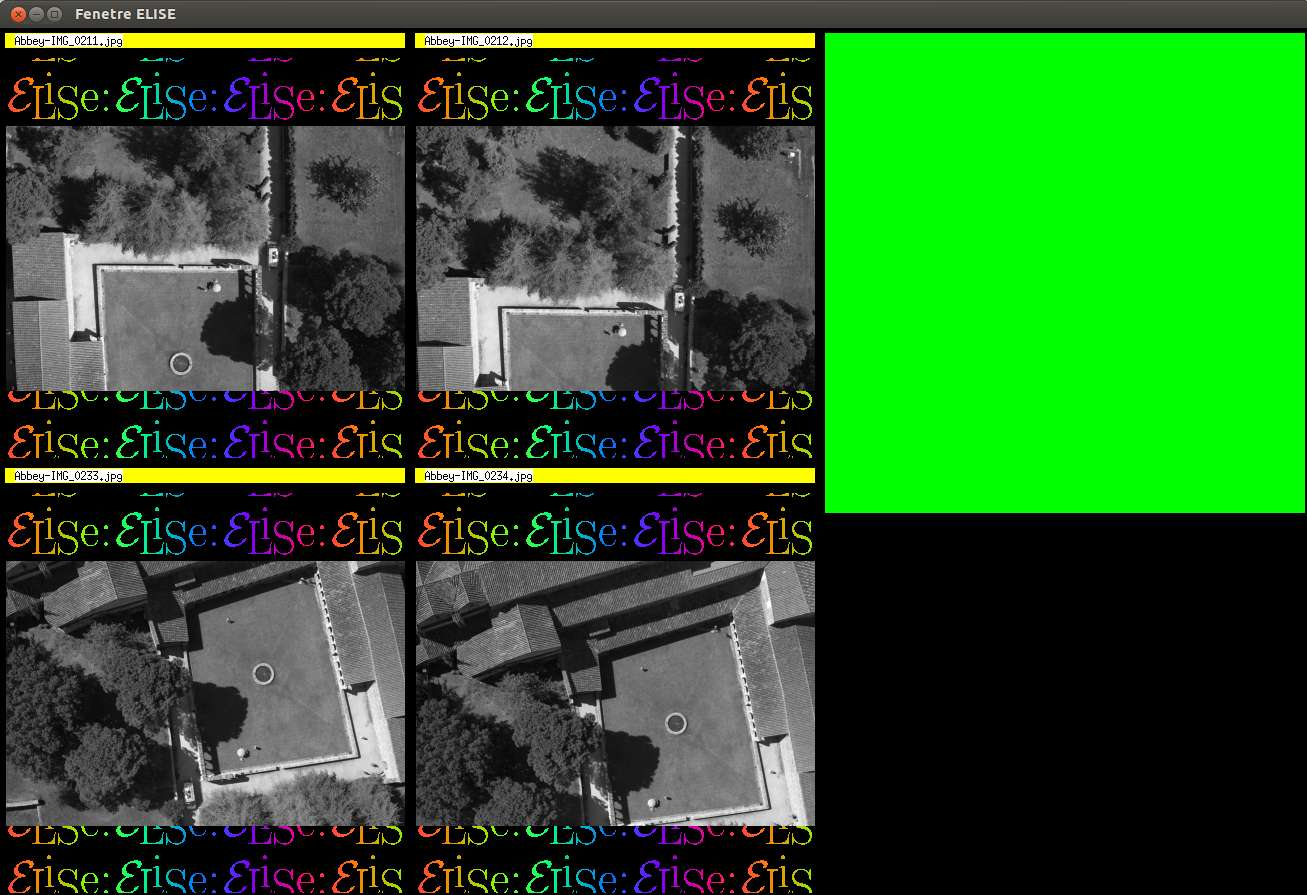
\includegraphics[width=160mm]{FIGS/Saisie/interface.jpg}
\end{center}
\caption{SaisieAppuis interface for ground control point selection}
\label{FIG:SaisieAppuis:interface}
\end{figure}

The general process for inputting ground control points is:
\begin{itemize}
\item Input a point in an image (Left-click)
\item Select its name,
\item Input the same point in the other images: move the yellow point and validate it with (right-clic + ;-) )
\item Iterate on each point you want to add (at each iteration, it can be useful after having pointed the point in one image to zoom on this point in all the images,
this can be done by (Ctrl + right-click + {\tt This Point})
\end{itemize}

When exiting the interface, two {\tt Xml} files are stored, with respectively 2D and 3D coordinates of input points.
Note that if for some reason some points are missing, you can re-run the same command, and continue the input job.
Points that have already been stored will be displayed, and the same process can be followed.\\

{\tt SaisieAppuisInit} is available on Linux and MacOS.
An equivalent tool is available on Windows, Linux and MacOS and is called with command: \begin{verbatim} mm3d SaisieAppuisInitQT + arguments \end{verbatim}
It runs with the same arguments as {\tt SaisieAppuisInit}. For example:
\begin{verbatim}
mm3d SaisieAppuisInitQT  "IMG_(023[3456]).jpg" All NamePoint.txt  Mesure.xml
\end{verbatim}

Same equivalent tools exist for {\tt SaisieAppuisPredic} and {\tt SaisieBasc} (ie. \begin{verbatim}mm3d SaisieAppuisPredicQT and mm3d SaisieBascQT\end{verbatim} ).

A visual interface for argument edition is also available with command: \begin{verbatim} mm3d vSaisieAppuisInitQT} or  mm3d vSaisieAppuisPredicQT \end{verbatim}

{\tt SaisieAppuisInitQT} displays two lists on the right side: the points list, and the images list. Points list can be clicked to choose which point to measure. You can also remove a point by clicking it in the list and press {\tt Suppr}. You can also right-click and choose between following actions: 
\begin{itemize}
\item Change images for selected point
\item Delete selected points (multiple selection allowed)
\item Validate selected points (idem)
\end{itemize}
The image lists show all available images. When a point has been measured in at least two images, the image list is displayed.
Images currently displayed in the windows are highlighted in blue. The image where the cursor is moving is displayed in light orange. You can right-click and select {\tt View images} to load corresponding images.
A 3D window shows the images location, and the point measured. By default point are displayed in red ; when a point is selected, it is displayed in blue.
You can drag-and-drop a ply file in this window (such as AperiCloud.ply) to check if GCP are good.

\begin{figure}[H]
\begin{center}
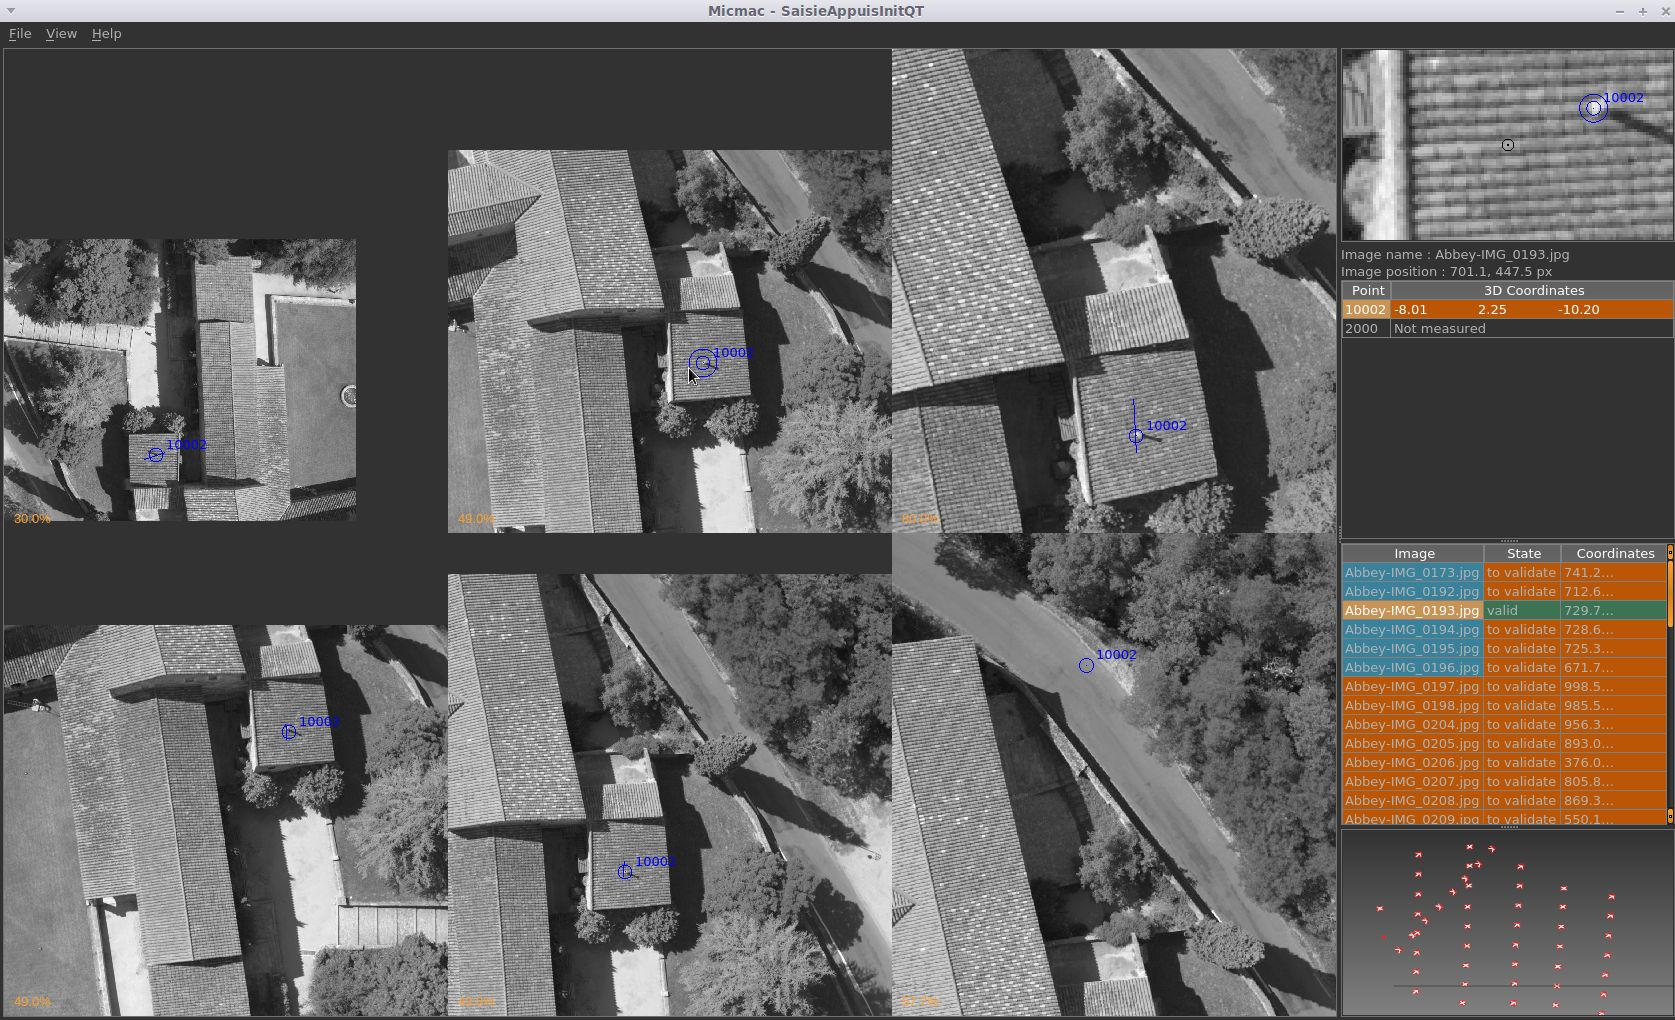
\includegraphics[width=160mm]{FIGS/Saisie/SaisieAppuisInitQT.jpg}
\end{center}
\caption{QT interface SaisieAppuisInitQT}
\label{FIG:SaisieAppuis:QT}
\end{figure}

\subsection{For fast predictive entering GCP with {\tt SaisieAppuisPredic}}

When enough points have been selected, interface can give a prediction for each new input:

\begin{figure}[H]
\begin{center}
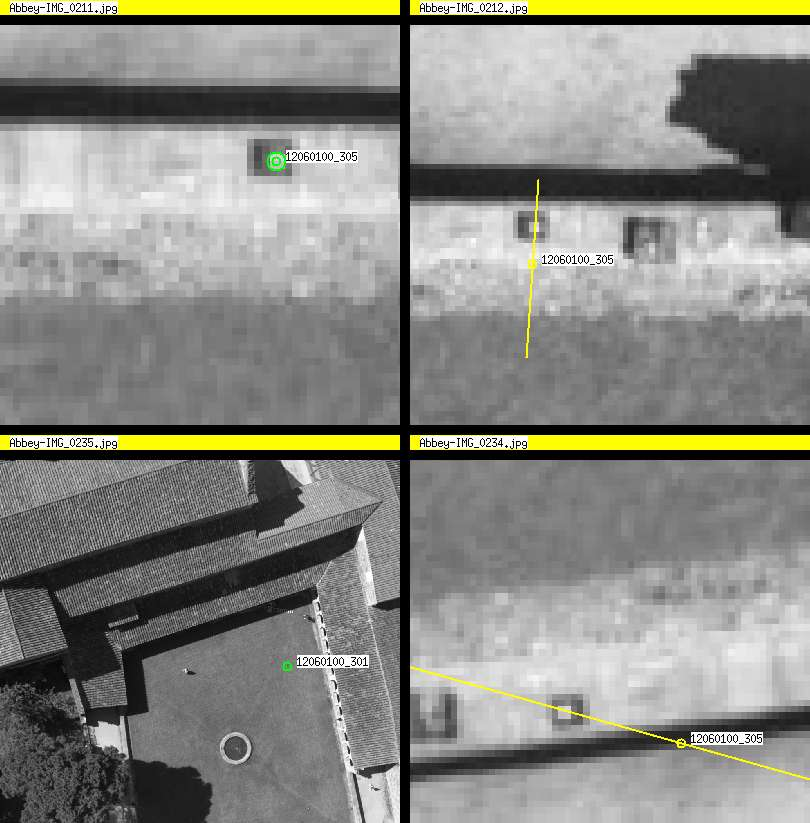
\includegraphics[width=120mm]{FIGS/Saisie/prediction.jpg}
\end{center}
\caption{Prediction help for adding new point}
\label{FIG:SaisieAppuis:prediction}
\end{figure}

 %  -  -  -  -  -  -  -  -  -  -  -  -  -
\subsection{For bascule with {\tt SaisieBasc}}
\label{SaisieBasc}

{\tt SaisieBasc} is a graphic interface to measure objects
to be able to perform transformations such as data scaling, rigid transformation (rotation, translation).\\*

One can size a point to set the origin of the new frame.
One can size two lines:
\begin{itemize}
\item one to set horizontal (with two points: Line1, Line2)
\item one to set scale (with two points: Ech1, Ech2)
\end{itemize}


%=======================================

\section{Visualize Tie-points with {\tt SEL}}

An old and ugly tool, but it can help. To visualize tie points computed with
{\tt Tapioca} :

\begin{verbatim}
SEL  ./ Face2-IMGP5331.JPG Face2-IMGP5333.JPG KH=NB
\end{verbatim}

For creating a few set of tie points and save in XML format :

\begin{verbatim}
SEL  ./ Face2-IMGP5331.JPG Face2-IMGP5333.JPG KH=S
\end{verbatim}


%=======================================
\COM{

\section{Generating auxiliary ply visualisation}


\subsection{PlySphere}

To visualize a single point in a ply format, use {\tt PlySphere} :

\begin{verbatim}
mm3d TestLib PlySphere -help
*****************************
*  Help for Elise Arg main  *
*****************************
Mandatory unnamed args : 
  * Pt3dr :: {Center of sphere}
  * REAL :: {Ray of sphere}
Named args : 
  * [Name=NbPts] INT :: {Number of Pts / direc (Def=5, give 1000 points)}
\end{verbatim}


\subsection{San2Ply}

To visualize an analytcal surface (currently a cylinder) in fly format, use {\tt San2Ply} :

\begin{verbatim}
mm3d TestLib PlySphere -help
*****************************
*  Help for Elise Arg main  *
*****************************
Mandatory unnamed args : 
  * Pt3dr :: {Center of sphere}
  * REAL :: {Ray of sphere}
Named args : 
  * [Name=NbPts] INT :: {Number of Pts / direc (Def=5, give 1000 points)}
\end{verbatim}


llll
}






